\section{Conduction of the experiment}
After the entrance exam the distances on the lid of the Dewar with the SQUID probe and the distance between the top of the Dewar and the position of the sample to later be able to compute the distance between the sample and the sensor. All distances were measured thee times to reduce the measurement inaccuracy. After that was finished, the Dewar was filled with the liquid nitrogen and the SQUID probe was placed inside to cool it down. While the sensor is cooling, the loop of the resistor measurements was measured from different angles because it is quite asymmetric. \par
Now, after approx. 15 minutes, the VCA and VCO settings in the control software of the SQUID were set as a calibration. They were modified so the SQUID signal has, as seen in figure \ref{cali_squid}, the characteristic differences from the usual sine function at the maxima and minima of the triangular reference voltage are as visible as possible.

\begin{figure}[ht]
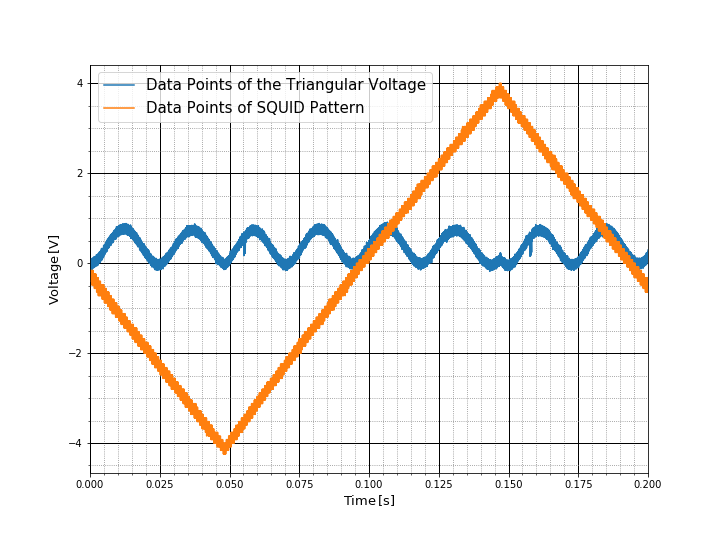
\includegraphics[scale=0.5]{Bild/Eichung}
\centering
\caption[Picture of the calibration of the SQUID]{\small The figure shows the SQUID signal after being calibrated for the measurement. }
\label{cali_squid}
\end{figure}
\par
Now, after measuring the battery voltages, the measurements for the resistors were conducted. Starting with the smallest, four measurements of every resistor for each used motor speed were made. For the first resistor, the speed settings 10, 5 and 2 were used. During the measurements of the second resistor, it became clear that measurements of with the speed of 2 are not viable due to an increase in background interference. For the other resistors, only the speeds 10 and 5 were used and, also due to the increased background instabilities, only thee measurements each were made. After finishing the resistor measurements, the rotational speed of the motor settings 10 and 5 was measured over multiple rotations.\par
Now five different other samples were measured, each at a speed set to 10. The samples can be seen in figure \ref{samples} First a iron splinter, which worked well. Second a gold plate was tried, which did unfortunately not seem to have any measurable dipole moment. After taking two measurements, the signal suddenly disappeared and it seemed like, nothing was inside of the SQUID apparatus.Because there was a signal, the measurement should be retried later. The third sample was a magnet splinter, which also worked well.
After that, the gold sample was retried, and still no signal was measurable. Now, a stone was measured. After this, the gold sample was retried one last time, but it still showed no signal at all. As a last sample, a magnet was measured. It was chosen as the last sample, because it influences the detector so strong that for the rest of the day no other measurements can be made. \par
As the last measurement, the resistors were measured with the multimeter.

\begin{figure}[ht]
	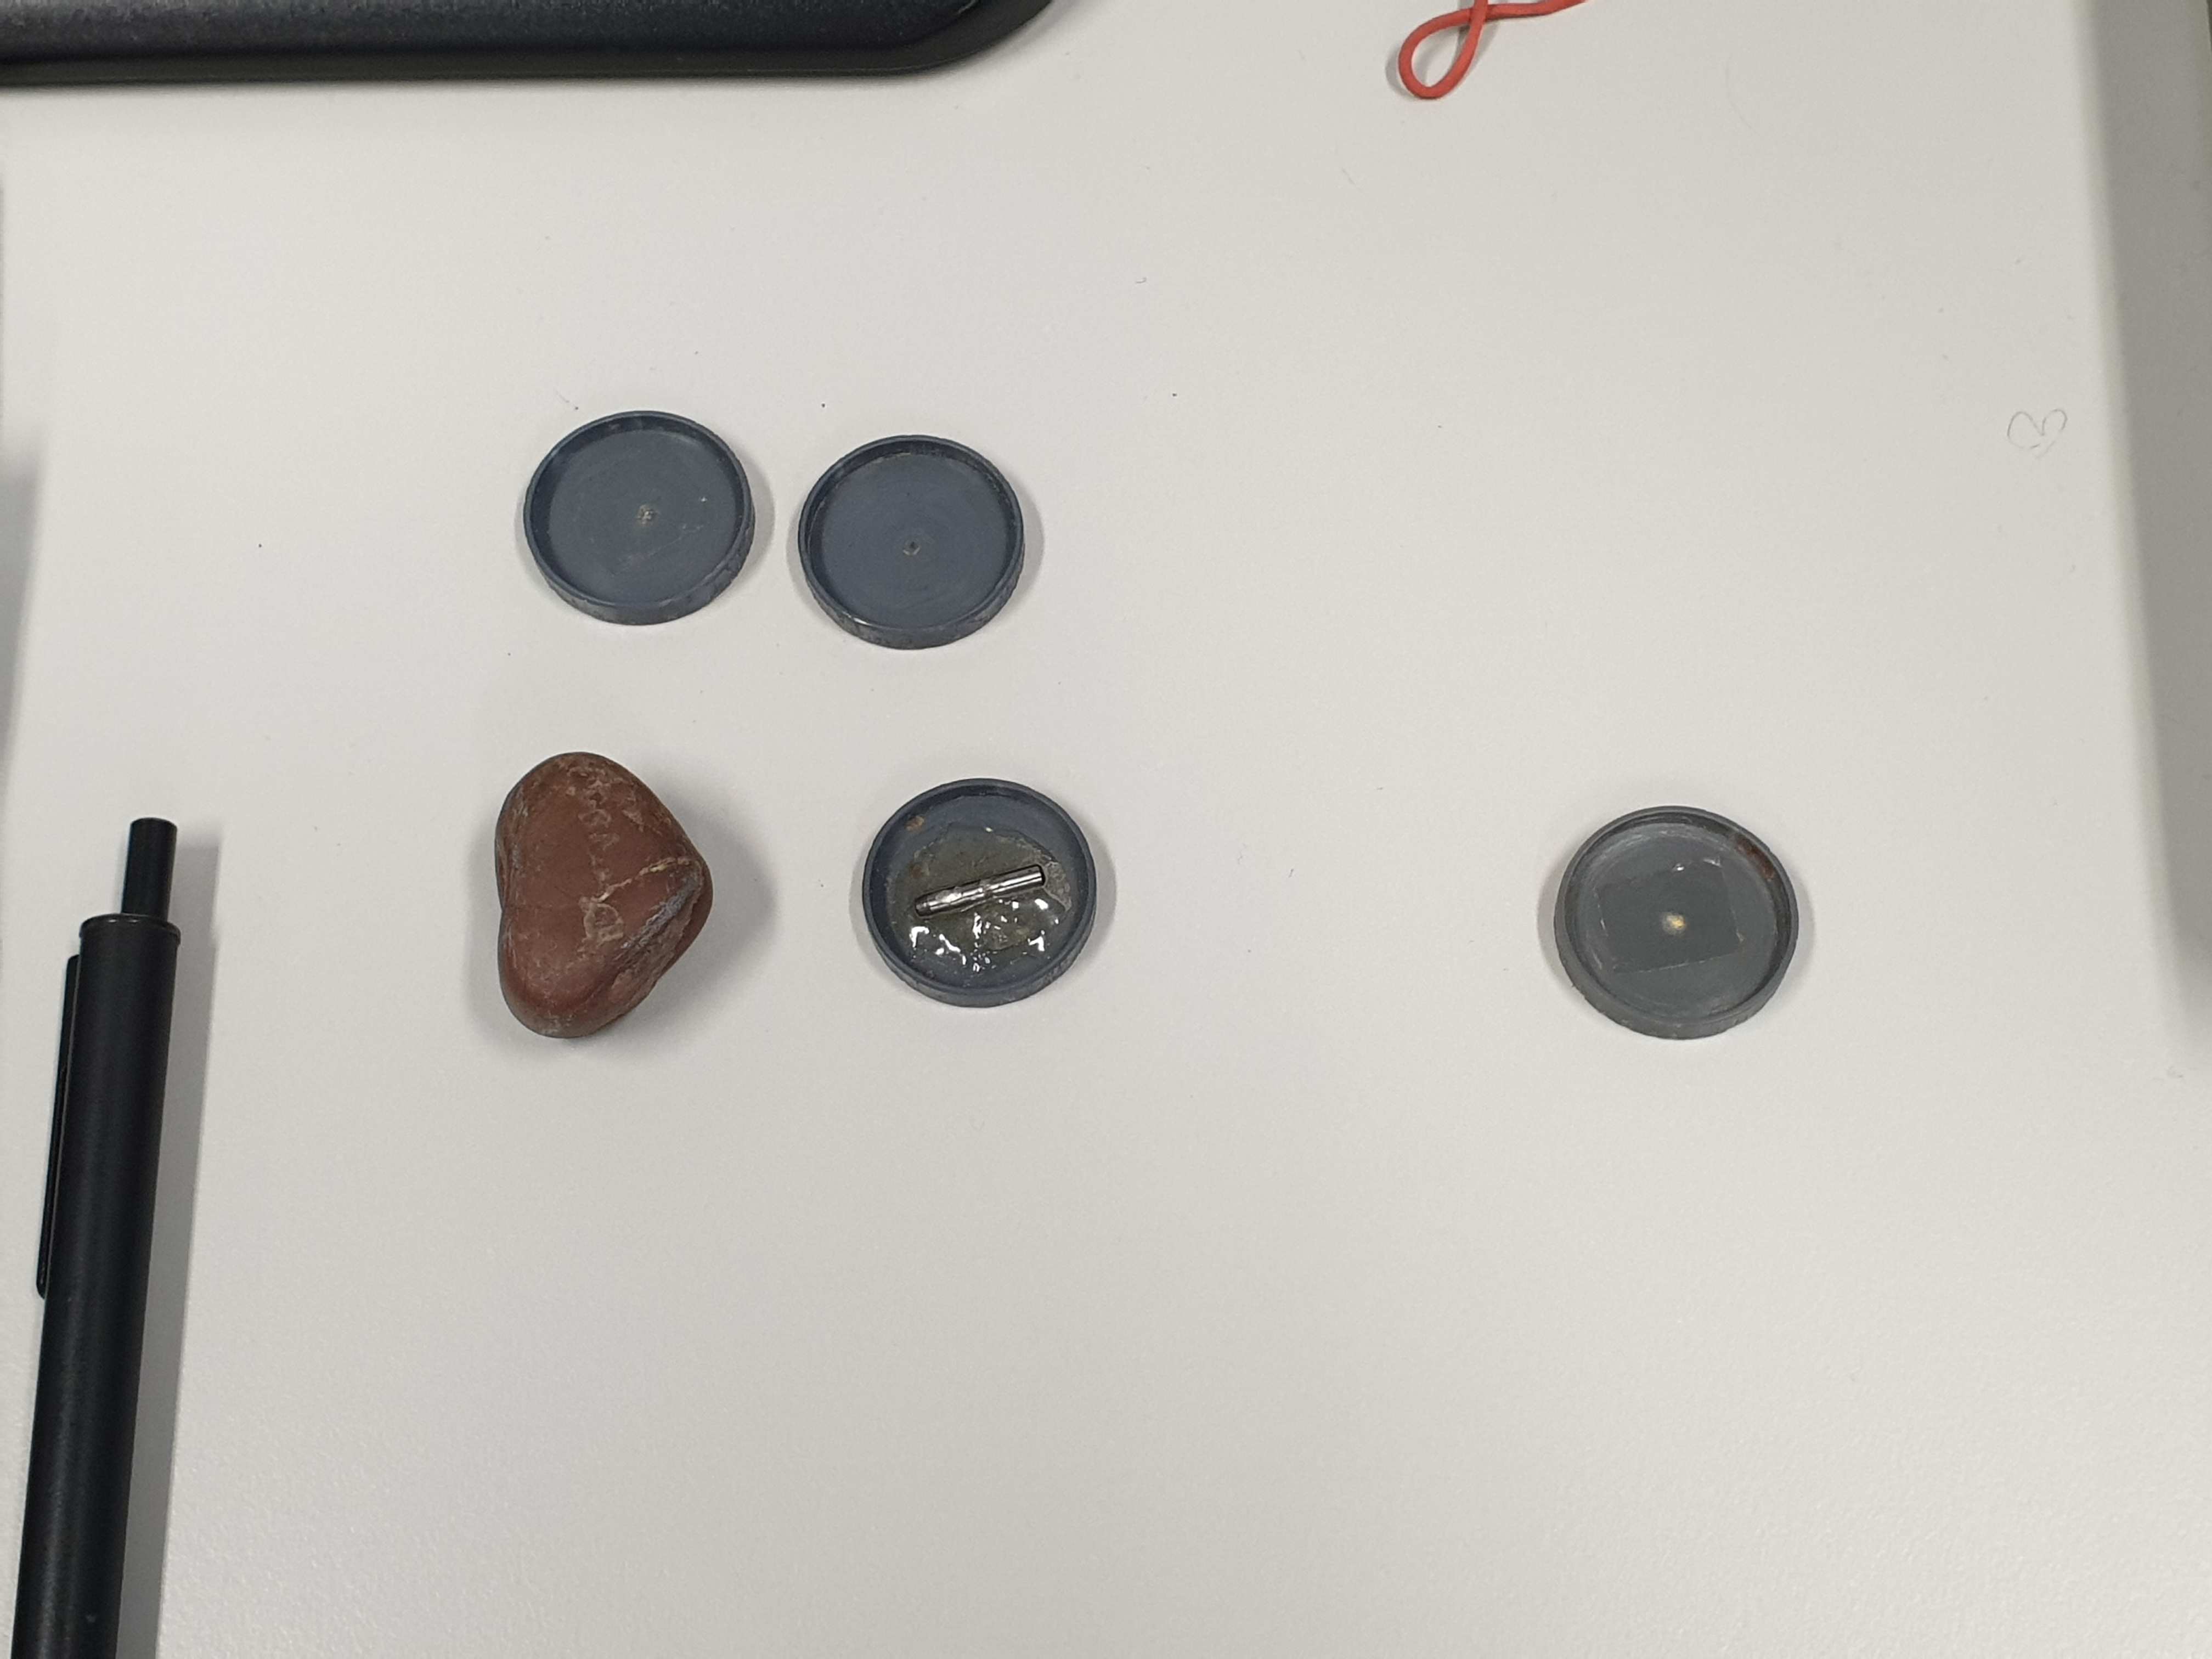
\includegraphics[scale=0.1,angle=0]{Bild/samples}
	\centering
	\caption[Picture of the other samples]{\small The picture shows the other five samples used during the experiment. In the quadratic arranged samples, the top right one is the iron splinter, the top left is the magnet splinter. The bottom left one is the stone, the bottom right one is the magnet. To the right of the other samples, the gold sample is placed.}
	\label{samples}
\end{figure}